\begin{frame}
\frametitle{Conditions and data}

\begin{table}[h!]
\caption{Conditions and data for run \runNumber}
\begin{center}
\begin{tabular}{|c|c|}
\hline
Conditions & Data \\
\hline
run number & \runNumber \\
file range & (0,4621) \\
date & 2021-06-07 \\
lab temperature: & 20.4 $\deg$ \\
Total number of S2s  &  1230687 \\
Total number of events & 1203762 \\
\hline
\end{tabular}
\end{center}
\label{r\runNumber.data}
\end{table}%
\end{frame}

\begin{frame}
\begin{figure}
  \begin{center}
      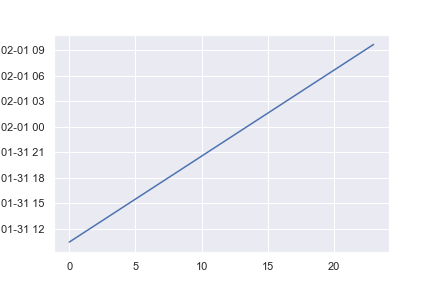
\includegraphics[width=0.45\textwidth]{img/r\runNumber _st200819/runTime.png}
      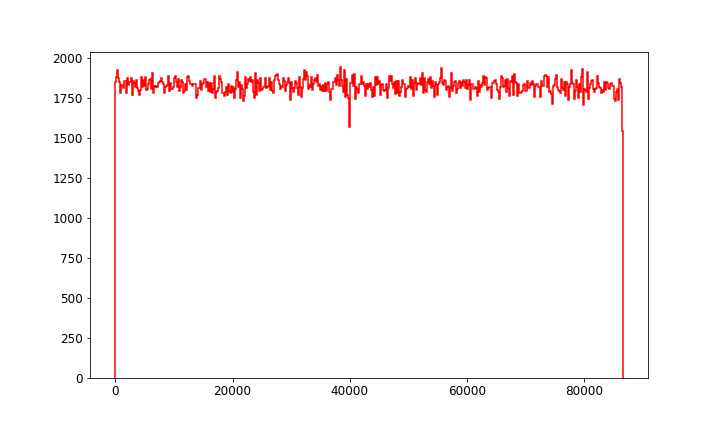
\includegraphics[width=0.45\textwidth]{img/r\runNumber _st200819/runEvt.png}
    \caption{Run data.}
  \end{center}
\end{figure}
\end{frame}

\begin{table}[h!]
\caption{S1 \& S2 for run \runNumber}
\begin{center}
\begin{tabular}{|c|c|}
\hline
Conditions & Data \\
\hline
fraction of S1s & 0.87 \\
fraction of S2s (1 S1) & 0.98 \\
fraction 1 S2 \& 1 S1 & 0.85 \\
\hline
\end{tabular}
\end{center}
\label{r\runNumber.data}
\end{table}%

\begin{frame}
\begin{figure}
  \begin{center}
      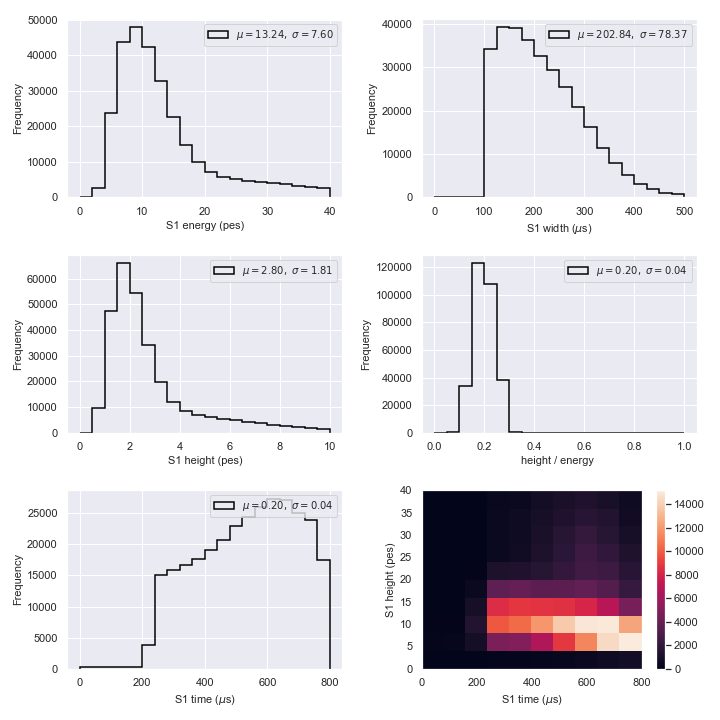
\includegraphics[width=0.6\textwidth]{img/r\runNumber _st200819/s1.png}
    \caption{S1 distributions.}
  \end{center}
\end{figure}
\end{frame}

\begin{frame}
\begin{figure}
  \begin{center}
      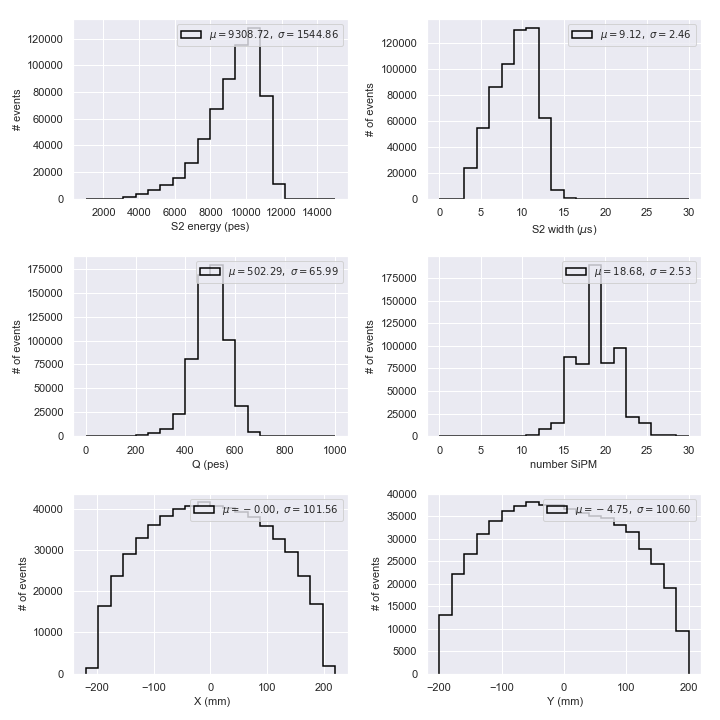
\includegraphics[width=0.6\textwidth]{img/r\runNumber _st200819/s2.png}
    \caption{S2 distributions.}
  \end{center}
\end{figure}
\end{frame}

\begin{frame}
\frametitle{Control distributions}
\begin{figure}
  \begin{center}
      \includegraphics[width=1\textwidth]{img/r\runNumber _st200819/EventDist_\runNumber .png}
    \caption{XYZ distribution.}
  \end{center}
\end{figure}
\end{frame}

\begin{frame}
\frametitle{Lifetime maps}
\begin{figure}
  \begin{center}
      \includegraphics[width=0.7\textwidth]{img/r\runNumber _st200819/lt_e0_xy_\runNumber .png}
    \caption{Lifetime and geometrical map.}
  \end{center}
\end{figure}
\end{frame}

\begin{frame}
\frametitle{Lifetime maps}
\begin{figure}
  \begin{center}
      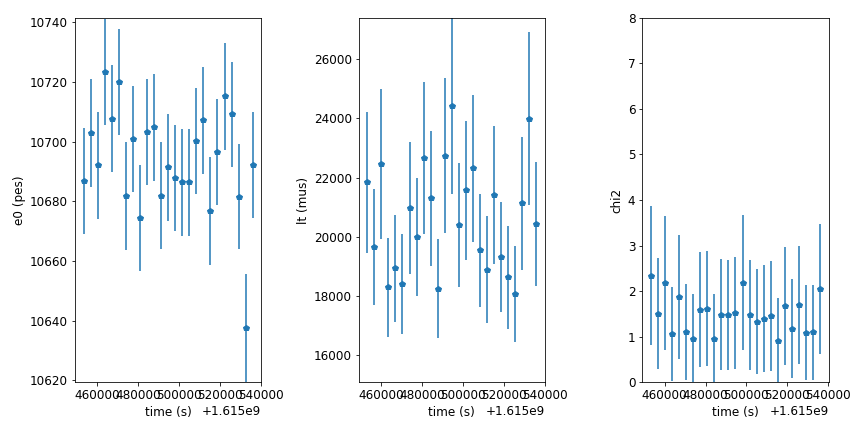
\includegraphics[width=0.7\textwidth]{img/r\runNumber _st200819/AverageLT.png}
    \caption{Average lifetime.}
  \end{center}
\end{figure}
\end{frame}

\begin{frame}
\frametitle{Lifetime and geometry correction}
\begin{figure}
  \begin{center}
      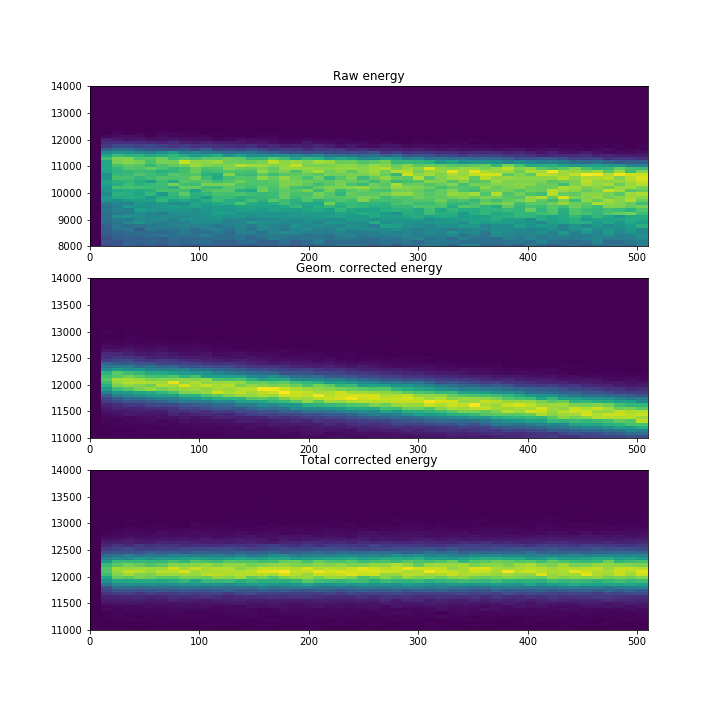
\includegraphics[width=0.7\textwidth]{img/r\runNumber _st200819/CorrectionLT.png}
    \caption{Lifetime and geometry correction.}
  \end{center}
\end{figure}
\end{frame}

\begin{frame}
\frametitle{R Profile showing R dropout}
\begin{figure}
  \begin{center}
      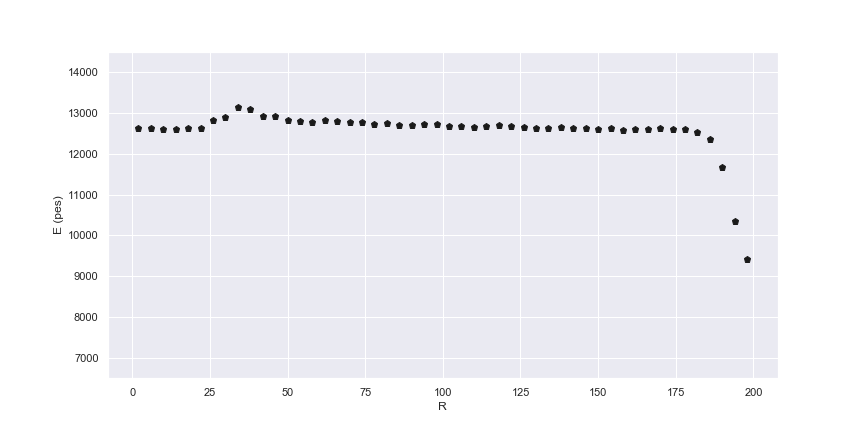
\includegraphics[width=0.7\textwidth]{img/r\runNumber _st200819/RProfile.png}
    \caption{R profile shows that fiducial volume must be $R < 180$mm.}
  \end{center}
\end{figure}
\end{frame}


\begin{frame}
\frametitle{Profiles after $R < 180$mm}
\begin{figure}
  \begin{center}
      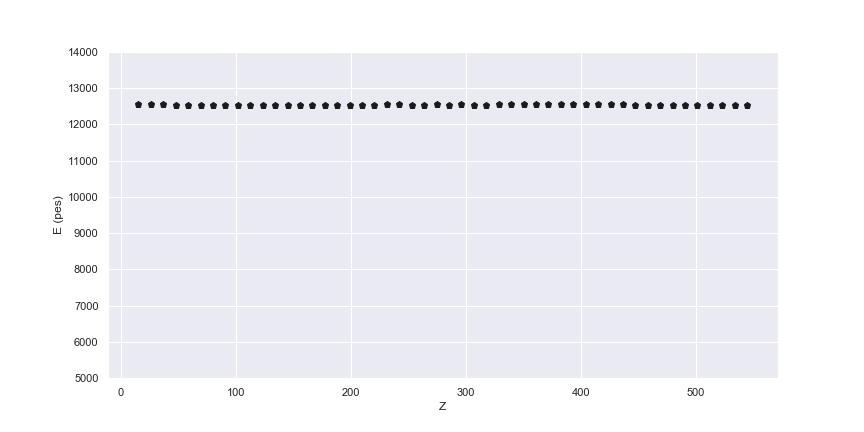
\includegraphics[width=0.4\textwidth]{img/r\runNumber _st200819/ZProfile.png}
      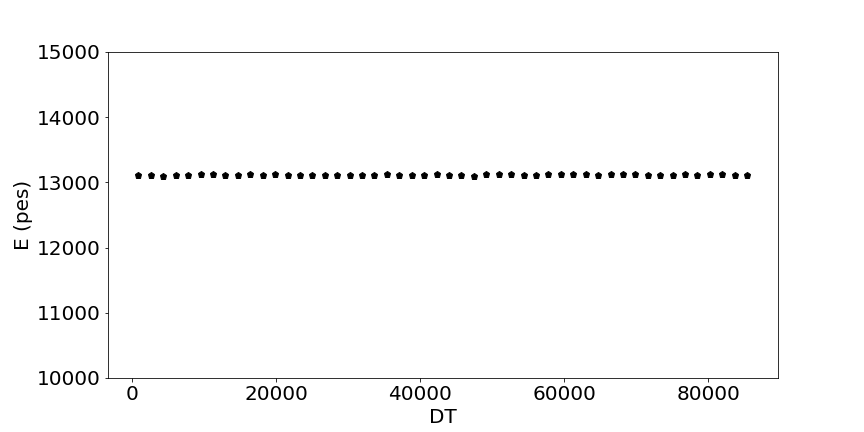
\includegraphics[width=0.4\textwidth]{img/r\runNumber _st200819/TProfile.png}
    \caption{Profiles showing correction is robust.}
  \end{center}
\end{figure}
\end{frame}

\begin{frame}
\frametitle{Resolution fits as a function of R and Z}
\begin{figure}
  \begin{center}
      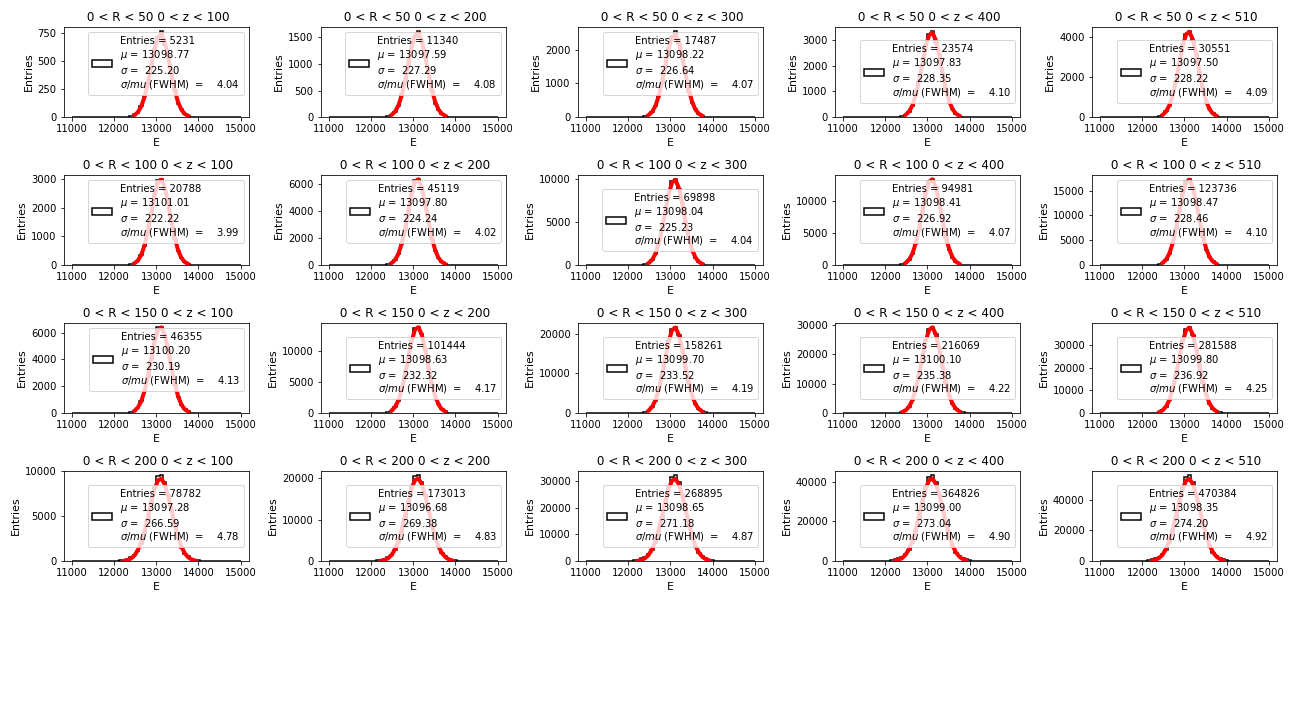
\includegraphics[width=0.8\textwidth]{img/r\runNumber _st200819/ResoFit.png}
    \caption{Resolution fits.}
  \end{center}
\end{figure}
\end{frame}

\begin{frame}
\frametitle{Resolution as a function of R and Z}
\begin{figure}
  \begin{center}
      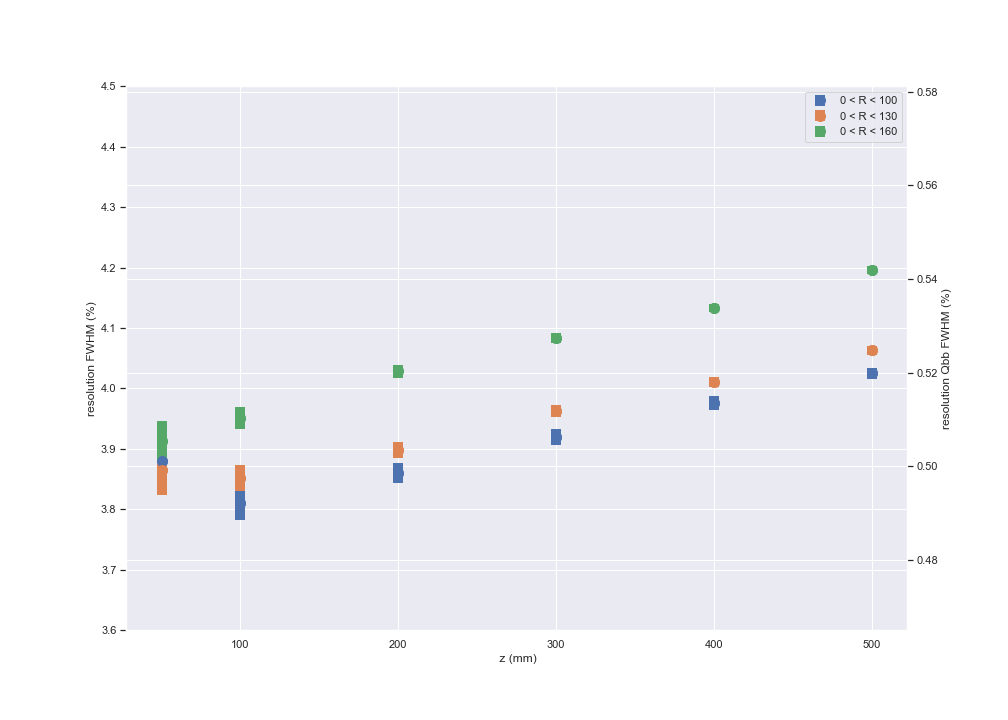
\includegraphics[width=0.8\textwidth]{img/r\runNumber _st200819/ResoVsZR.png}
    \caption{Resolution fits.}
  \end{center}
\end{figure}
\end{frame}

\begin{frame}
\frametitle{Efficiency over time}
\begin{figure}
  \begin{center}
      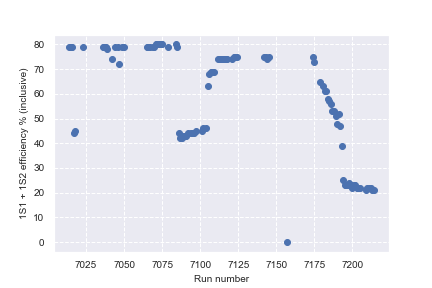
\includegraphics[width=0.8\textwidth]{img/r\runNumber _st200819/EffVsTime.png}
    \caption{Efficiency tracking over time.}
  \end{center}
\end{figure}
\end{frame}

\begin{frame}
\frametitle{Response over time}
\begin{figure}
  \begin{center}
      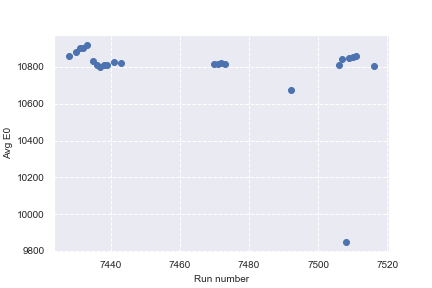
\includegraphics[width=0.8\textwidth]{img/r\runNumber _st200819/E0VsTime.png}
    \caption{Response tracking over time.}
  \end{center}
\end{figure}
\end{frame}

\begin{frame}
\frametitle{Lifetime over time}
\begin{figure}
  \begin{center}
      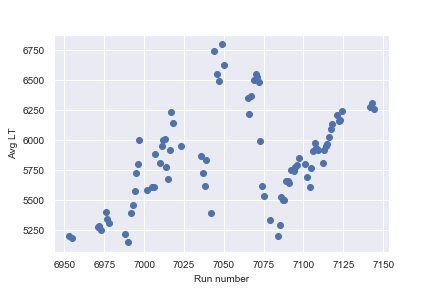
\includegraphics[width=0.8\textwidth]{img/r\runNumber _st200819/LTVsTime.png}
    \caption{Lifetime tracking over time.}
  \end{center}
\end{figure}
\end{frame}

\begin{frame}
\frametitle{Resolution over time}
\begin{figure}
  \begin{center}
      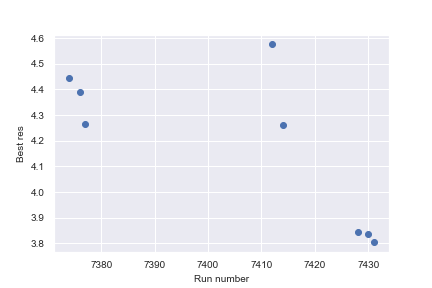
\includegraphics[width=0.8\textwidth]{img/r\runNumber _st200819/ResVsTime.png}
    \caption{Resolution tracking over time.}
  \end{center}
\end{figure}
\end{frame}
